\subsection{Diseño paramétrico}

El término \textit{paramétrico} se originó en las matemáticas, pero hay un debate sobre cuándo comenzaron los diseñadores a usar la palabra, David Gerber (2007, 73) en su tesis doctoral ``Parametric Practice'' acredita a Maurice Ruiter por usar el término en un trabajo de 1988 titulado ``Parametric Design''. En 1998 la compañía Parametric Technology Corporation, fundada por el matemático Samuel Geisberg lanzó el primer software de modelado paramétrico con éxito comercial: Pro / ENGINEER (Weisberg 2008, 16.5). Por su parte, Robert Stiles (2006) sostiene que la verdadera procedencia del término se produjo décadas antes en los escritos de los años 40 por el arquitecto Luigi Moretti (Bucci y Mulazzani 2000, 21).\vskip
Moretti (1971, 207) escribió extensamente sobre la arquitectura paramétrica, que define el estudio de los sistemas de arquitectura con el objetivo de ''definir las relaciones entre las dimensiones que dependen de los diversos parámetros''. Moretti usó el diseño de un estadio como un ejemplo, explicando cómo la forma del estadio puede derivar de diecinueve parámetros relacionados con aspectos como ángulos de visión y el costo económico del hormigón.\vskip
Sin embargo, la parametrización tiene una larga historia en las matemáticas y los ejemplos más antiguos que se encontraron para describir modelos tridimensionales se producen casi cien años antes de los escritos de Moretti. 
Un ejemplo es el artículo de James Dana sobre el dibujo de figuras de cristales de 1837 (otros ejemplos del período incluyen: Leslie 1821, Earnshaw 1839) [2]. En el documento, Dana explica los pasos generales para dibujar una gama de cristales y las disposiciones para las variaciones utilizando un lenguaje mezclado con parámetros, variables y proporciones. Dana 1837, 42 \vskip

\begin{figure}
\centering
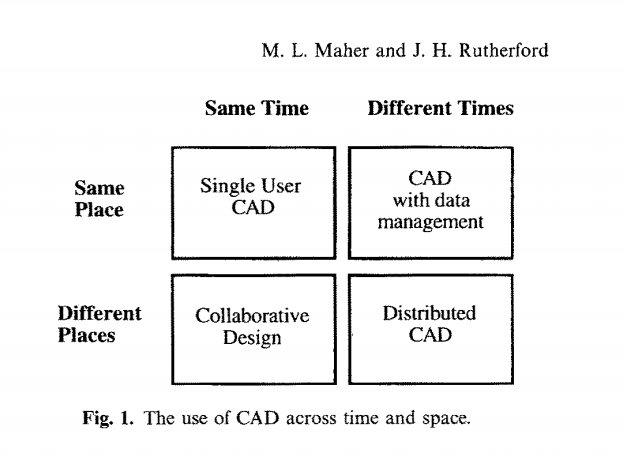
\includegraphics[width=12cm]{Img/CPD/2-CAD.png}
\caption[(optional short caption)]{\label{us_figure} DANA}
\end{figure}


Existen muchos otros casos de ciencia del principio del siglo XIX involucrados con las matemáticas de representaciones paramétricas. Un ejemplo de esa época incluye a Sir John Leslie (1821, 390), en su libro sobre análisis geométrico, demostrando la auto-similitud de las curvas catenarias usando "círculos paramétricos". Otro ejemplo es el de Samuel Earnshaw (1839, 102), que escribió sobre "superficies paramétricas hiperbólicas" deformadas por líneas de fuerza en un documento que dio lugar al teorema de Earnshaw. Estos ejemplos de expresar la geometría con ecuaciones paramétricas son dos de muchos del período, un período mucho antes de que Antoni Gaudí comenzara a diseñar arquitectura con curvas catenarias paramétricas y paraboloides hiperbólicos paramétricos a fines del siglo XIX.

Es imposible saber si Gaudí fue influenciado directamente por los científicos y matemáticos que anteriormente habían utilizado ecuaciones paramétricas para definir geometrías. Mark Burry (2007a, 11), el actual arquitecto ejecutivo de la Sagrada Familia de Gaudí, explica que ``prácticamente no hay nada escrito por el propio Gaudí sobre las motivaciones, las teorías y la práctica que lo llevaron a estirar los límites'' a pesar de que currículum universitario de Gaudí incluía, entre otras cosas, "matemáticas avanzadas, física general, ciencias naturales y geometría descriptiva" (Català 2007, 81). La comprensión profunda de Gaudí sobre las matemáticas es la base de su arquitectura, especialmente en sus trabajos posteriores, que consiste en superficies diseñadas con helicoides, paraboloides e hiperboloides paramétricamente asociados con superficies regladas, booleanos, relaciones geométricas y arcos catenarios (J. Burry y M Burry 2010, 35 - 39, M. Burry, 2011, 144). \cite{Davis2013}

Mark Burry (2011) plantea que uno de los primeros ejemplos es la maqueta que utilizó el arquitecto para representar el modelo de la cripta de la Colonia Guell, a principios del siglo XX. Este modelo estaba compuesto por cadenas que sostenían pesos, y actuaban por la fuerza de la gravedad.
La maqueta fue realizada al revés, y Gaudí le sacó una fotografía para poder visualizarla al derecho. Una cadena que cuelga tiene por lo menos cuatro parámetros: su longitud, su peso y los dos puntos a los que está sujetada. La cadena colgando a la merced de la fuerza de la gravedad adopta una forma curva. Esta curva es la función explicita de los parámetros de la cadena, con la propiedad agregada de que cuando es invertida la curva actúa por pura compresión. Al no haber una computadora, la cadena colgante es un modelo paramétrico gracias a la presencia de parámetros que controlan una forma derivada de una función explicita (en este caso, calculada por la gravedad).



El \textbf{Diseño Paramétrico} se entiende en términos generales como un proceso de descripción de una problemática utilizando variables. Actualmente para describir estas variables, los diseñadores
insertan valores numéricos o algoritmos en un software especializado, y al cambiar las
variables se generan una serie de alternativas de soluciones, y según el criterio del diseñador, la solución final es creada. Davis (2013) y Hudson (2010) concuerdan en que el diseño paramétrico en su definición contemporánea es únicamente posible creando un \textbf{modelo paramétrico}. Esto lo definen como un conjunto de ecuaciones que expresan una geometría explícitamente por medio de funciones definidas por parámetros. Esta representación se basa en las relaciones entre estas variables. Todo sistema de esta índole está compuesto por unos parámetros iniciales y las relaciones entre ellos, de manera que si se ajusta uno de los parámetros, el resultado se verá afectado de manera acorde, al igual que si se altera alguna de las relaciones. Esto brinda una característica de fuerte y sencilla maleabilidad, que permite verificar resultados fácilmente. El diseñador que emplea estas herramientas en vez de diseñar un objeto resultante, se enfoca en crear lógicas que pongan en relación estos parámetros y resulten en un sistema vivo y ampliamente modificable de acuerdo al criterio del diseñador, asistido por la
computadora. El uso de este método por medio de la manipulación de los sistemas fomenta la exploración y la experimentación de las formas del producto, que se generan automáticamente por la modificación de los parámetros o las relaciones. Woodbury (2010) afirma que el diseño es cambio y que el modelado paramétrico representa el cambio. Esto lo menciona como una característica esencial del diseño paramétrico, como aquello que lo distingue de los métodos de diseño tradicionales. Es marcar e identificar las partes y como se relacionan y cambian de manera coordinada. (Woodbury, 2010). La demostración explicita de las partes es lo que contribuye a la intervención y modificación
interactiva en tiempo real, debido a la operatividad visible del cambio en el sistema. La
lógica sistemática del diseño paramétrico permite evaluar las relaciones de manera visible, en lugar de hacerlo de manera intuitiva por medio de un proceso mental interno.
Esto le permite al diseñador explorar y descubrir nuevas posibilidades en lugar de hurgar en sus conocimientos previos para llegar con una solución que ya conocía (Cross, 2006).
El autor también afirma que es necesaria una representación visual ya que diseñar es difícil de conducir puramente por procesos mentales internos (Cross, 2011, p. 12).\vskip
 


\begin{figure}
\centering
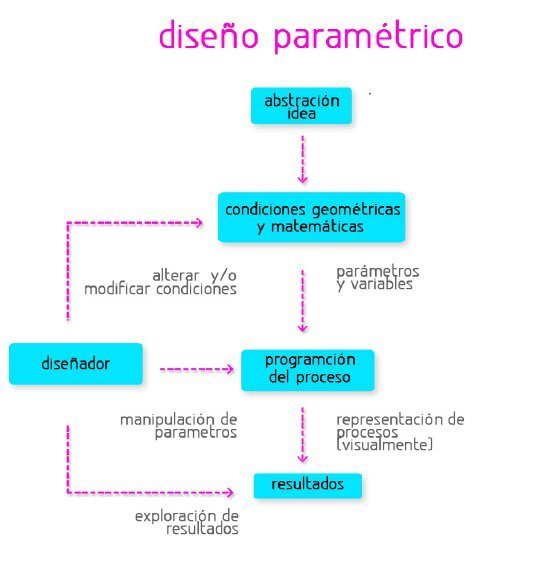
\includegraphics[width=12cm]{Img/CPD/4-PARAM.jpg}
\caption[(optional short caption)]{\label{us_figure} Proceso de diseño paramétrico }
\end{figure}


\subsection{CAD Paramétrico}

La innovación del modelo de Gaudí explicado en el punto 2.1.4 radica en que este calcula automáticamente los resultados, ya que al mover un parámetro se afecta todo el modelo, que a pesar de ser análogo, marcó el inicio de la actualización en tiempo real de geometrías con bases matemáticas, lo cuál le da el énfasis utilitario de explorar las
posibilidades que el modelo ofrece (ver Figura 1, pg. 95, anexo de imágenes seleccionadas).
Esto marcó la \textit{necesidad de facilitar la interacción entre el diseñador y el modelo}, que implicaba muchas representaciones manuales y modificaciones completas con cada cambio. No fue hasta la aparición de las computadoras y el primer programa CAD, 29 Sketchpad de Ivan Sutherland en 1963 que se facilitó la interacción en tiempo real del diseñador y la computadora. Yüksel (2014) lo describe como un sistema que tenía un puerto de entrada con un modelo de límites que promovía la interacción, porque al manipular una parte del modelo afectaría los cambios geométricos en otro. En el contexto de aparición de este programa, el proceso de diseño era enteramente manual y análogo,
donde un cambio mínimo significaría comenzar de nuevo. Al representar las geometrías en dos dimensiones en la computadora se facilitaba el proceso de diseño. A partir de esto se fueron desarrollando un amplio número de software cuyas capacidades y posibilidades se extendían con aquellas del procesamiento de datos de las
computadoras.
El recorrido histórico del desarrollo de software excede los objetivos de este trabajo final, pero la bifurcación entre el diseño computacional y la computarización del diseño es esencial para la compresión de los capítulos a seguir. Ambos términos suelen ser tomados como iguales, definidos como el uso de tecnologías CAD para realizar un
proyecto de diseño. La diferencia radica en su empleo. La computarización del diseño apunta a el uso de la computadora como herramienta de dibujo o representación formal de un proyecto concebido en la mente del diseñador, mientras que el diseño computacional aborda el diseño con bases en el pensamiento algorítmico, lo que engloba al diseño paramétrico y generativo. Otra de las interpretaciones incorrectas que se le da
al termino de diseño computacional es que su único uso es para crear formas complejas, y uno un proyecto final interactivo (Yüksel, 2014). Esta diferenciación puede apreciarse claramente en el modelo de Gaudí y el programa de Sutherland. La maqueta de Gaudí encarna un sistema de complejo de parámetros y relaciones, mientras que el programa
de Sutherland representa geometrías modificables. El diseño computacional se beneficia de la tecnología disponible, y al incorporar este método de pensamiento al proceso de diseño se involucra a la máquina como parte del proceso de generación de ideas, y no solo como un medio al que se le carga un diseño terminado para generar una imagen.

\textcolor{red}{


https://shapediver.com/m/mesa-auxiliar-2017-08-23


En este trabajo se optó por la utilización de modelos 3D paramétricos como medio indispensable para lograr la colaboración. Es indispensable que los diseños se generen en función de sus parámetros y además expongan sus características de manera comprensible por todas las partes involucradas. Por ejemplo: un diseñador industrial puede comprender naturalmente parámetros como arista, vértices o normales pero un artista puede comprender sobre dimensiones, colores o materiales. Por ende es recomendable que los modelos 3D en este caso se expongan en función de los parámetros conocidos por el artista.}
\textcolor{red}{Para ello surge la necesidad de mecanismos de manipulación directa de los modelos 3D por parte de los interesados para posibilitar la generación de nuevas soluciones, y así gracias al diseño iterativo lograr la colaboración.}



\subsection{CAD especificado en algoritmos} 
El diseño paramétrico también es posible a través de las interfaces de secuencias de comandos del inglés \textit{scripting}. Las interfaces de scripting permiten a los diseñadores escribir código para automatizar partes del software. Los desarrolladores de software como AutoCAD, incluso en 1982, se dieron cuenta de que la inclusión de estas interfaces les permitía <<Evitar muchas cosas personalizadas de codificación y aplicación que de lo contrario se les pediría>> (Walker 1994, 115). Diez años más tarde, en 1992, cuando Mark Burry (2011, 28-29) quería modelar las hipérbolas paramétricamente para la Sagrada Familia, en lugar de pedirle a Autodesk que incluyera una función de hipérbola en AutoCAD, utilizó la interfaz de scripting de AutoCAD para desarrollar la suya propia. El script de Burry tenía tres parámetros de entrada: un punto de origen, un punto mínimo y un punto de asíntoto. Estos parámetros se alimentan a través de una serie de ecuaciones explícitas (escritas en código AutoLISP) para emitir una hipérbola. 

El script, con sus parámetros de entrada, funciones explícitas y salidas, es una realización arquetípica de la definición matemática de paramétrico. Ipek Dino (2012, 210) ha argumentado que los scripts son inherentemente paramétricos, observando que "los sistemas paramétricos se basan principalmente en principios algorítmicos" ya que "un algoritmo toma un valor o un conjunto de valores como entrada, ejecuta una serie de pasos computacionales que transforman la Y finalmente produce un valor o un conjunto de valores como salida ". Por lo tanto, las interfaces de secuencias de comandos accesibles en la mayoría de los paquetes de software están innatamente predispuestas a crear modelos paramétricos.

Un ejemplo de uso de estas interfaces se puede encontrar en OpenSCAD. OpenSCAD es una aplicación libre para crear objetos sólidos de CAD, realiza geometría constructiva de sólidos (CSG). No es un editor interactivo sino un compilador 3D basado en un lenguaje de descripción textual. Un documento de OpenSCAD especifica primitivas geométricas y define como son modificadas y manipuladas para reproducir un modelo 3D.

FREECAD ... ver como eganchar


En la última década se ha visto la aparición de un nuevo tipo de interfaz de secuencias de comandos, la interfaz visual. La programación visual implica representar programas no como texto, sino como diagramas. Un ejemplo es Grasshopper que se basa en gráficos (un nombre matemático para un tipo de diagrama de flujo) que mapean el flujo de relaciones desde parámetros, a través de funciones definidas por el usuario, concluyendo normalmente con la generación de geometría. Los cambios en los parámetros o las relaciones del modelo hacen que los cambios se propaguen a través de las funciones explícitas para volver a dibujar automáticamente la geometría. Como tal, son otra forma de crear un modelo paramétrico.

http://www.patrikschumacher.com/Texts/Design%20Parameters%20to%20Parametric%20Design.html

http://fernandoalonsoarchitect.blogspot.com.ar/2017/01/historia-del-diseno-parametrico.html

Las herramientas de diseño asistido por computadora CAD tradicionales fueron pensadas para un usuario, por ende tienen limitaciones para soportar el entorno de desarrollo colaborativo de productos CPD y de forma rápida como requiere el mercado. Actualmente el desarrollo de productos es el resultado de procesos colaborativos basados en la red, porque la mayoría de los proyectos requieren la cooperación entre actores distribuidos geográficamente. En un proceso de desarrollo distribuido, se necesita una comunicación efectiva y de alta velocidad. La mayoría de los errores de diseño se deben a la falta de comunicación entre los equipos de diseño distribuidos.
Los sistemas de información distribuída que se han aplicado para CPD se pueden clasificar en 3: web services, remote services y remote repositories.Los sistemas basados en web services tienen ventajas sobre los otros dos porque son relativamente sencillos de diseñar e implementar, reducen los problemas de la instalación de software y facilita la posibilidad de la colaboración. \cite{Nyamsuren2015}
